\unput{../../preamble}


\title{Computational Economics and the AI Revolution}



\author{John Stachurski}


\date{2025}


\begin{document}

\begin{frame}
  \titlepage
\end{frame}



\begin{frame}{Topics}

    \begin{itemize}
        \item Introduction
        \vspace{0.5em}
        \item ANNs and deep learning
        \vspace{0.5em}
        \item Stochastic approximation
        \vspace{0.5em}
        \item Dynamic programming and reinforcement learning
        \vspace{0.5em}
    \end{itemize}

\end{frame}



\begin{frame}{AI-driven scientific computing}

    AI is changing the world

    \begin{itemize}
        \item generative AI  (LLMs, image / music / video generators)
        \vspace{0.5em}
        \item image processing / computer vision
        \vspace{0.5em}
        \item speech recognition, translation
        \vspace{0.5em}
        \item scientific knowledge discovery
        \vspace{0.5em}
        \item forecasting and prediction 
        \vspace{0.5em}
        \item etc
    \end{itemize}

    \pause

        \vspace{0.5em}
        \vspace{0.5em}
        \vspace{0.5em}
    Plus killer drones, Skynet, etc.\ldots

    
\end{frame}

\begin{frame}
    

    Private AI investment in 2024:

    \begin{itemize}
        \item U.S. = \$109 billion 
        \vspace{0.5em}
        \item China \$9.3 billion 
        \vspace{0.5em}
        \item UK \$4.5 billion
    \end{itemize}

        \vspace{0.5em}
        \vspace{0.5em}
    Massive investments in 

    \begin{itemize}
        \item data centers
        \vspace{0.5em}
        \item GPUs
        \vspace{0.5em}
        \item software 
    \end{itemize}


\end{frame}





\begin{frame}
    \frametitle{Deep learning in two slides}
    
    Aim: approximate an unknown functional relationship
    %
    \begin{equation*}
        y = f(x)
        \qquad (x \in \RR^k, \; y \in \RR)
    \end{equation*}

    \Egs
    %
    \begin{itemize}
        \item $x = $ cross section of returns, $y = $ return on oil futures tomorrow
        \vspace{0.5em}
        \item $x = $ weather sensor data, $y = $ max temp tomorrow
    \end{itemize}
        \vspace{0.5em}
        \vspace{0.5em}

    Problem:

    \begin{itemize}
        \item observe $(x_i, y_i)_{i=1}^n$ and seek $f$ such that $y_{n+1}
            \approx f(x_{n+1})$
    \end{itemize}

\end{frame}


\begin{frame}

    Nonlinear regression: 

    \begin{enumerate}
        \item Choose function class $\{f_\theta\}_{\theta \in \Theta}$ 
            \vspace{0.4em}
        \item Minimize the MSE
            %
            \begin{equation*}
                \ell(\theta) := \sum_{i=1}^n (y_i - f_\theta(x_i))^2
                \quad \st \quad \theta \in \Theta
            \end{equation*}
    \end{enumerate}


    \pause
    \vspace{0.5em}
    In the case of ANNs, elements of $\{f_\theta\}_{\theta \in \Theta}$
    have a particular structure

    \begin{itemize}
        \item We discuss this structure soon
        \vspace{0.5em}
        \item Typically, $\theta \mapsto f_\theta(x)$ is smooth for all $x$
        \vspace{0.5em}
        \item MSE is a popular loss function but others are also used
    \end{itemize}

\end{frame}


\begin{frame}
    

    Minimizing a smooth loss functions  -- what algorithm?
    
    \begin{figure}
       \begin{center}
        \scalebox{0.15}{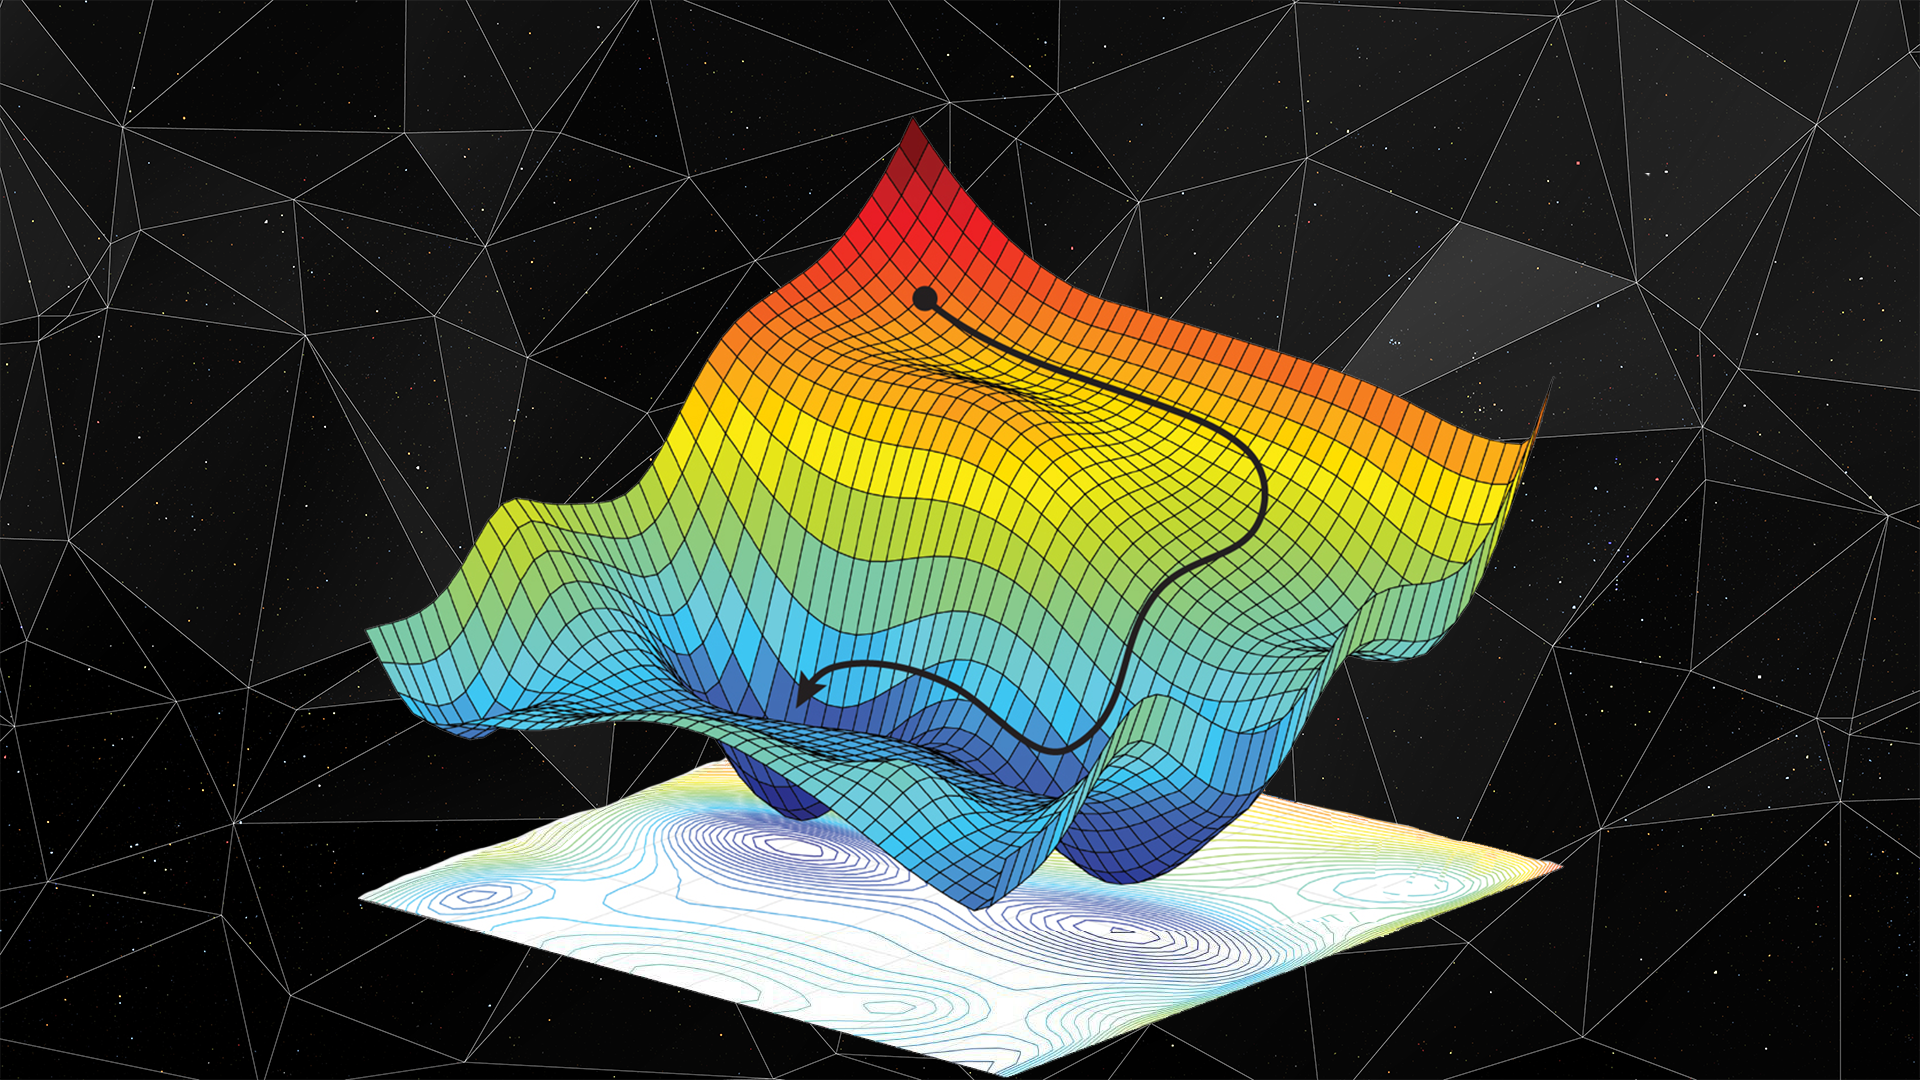
\includegraphics[trim={0cm 0cm 0cm 0cm},clip]{gdi.png}}
       \end{center}
    \end{figure}

    Source: \url{https://danielkhv.com/}

\end{frame}


\begin{frame}

    Deep learning: $\theta \in \RR^d$ where $d = ?$
    
    \begin{figure}
       \begin{center}
        \scalebox{0.14}{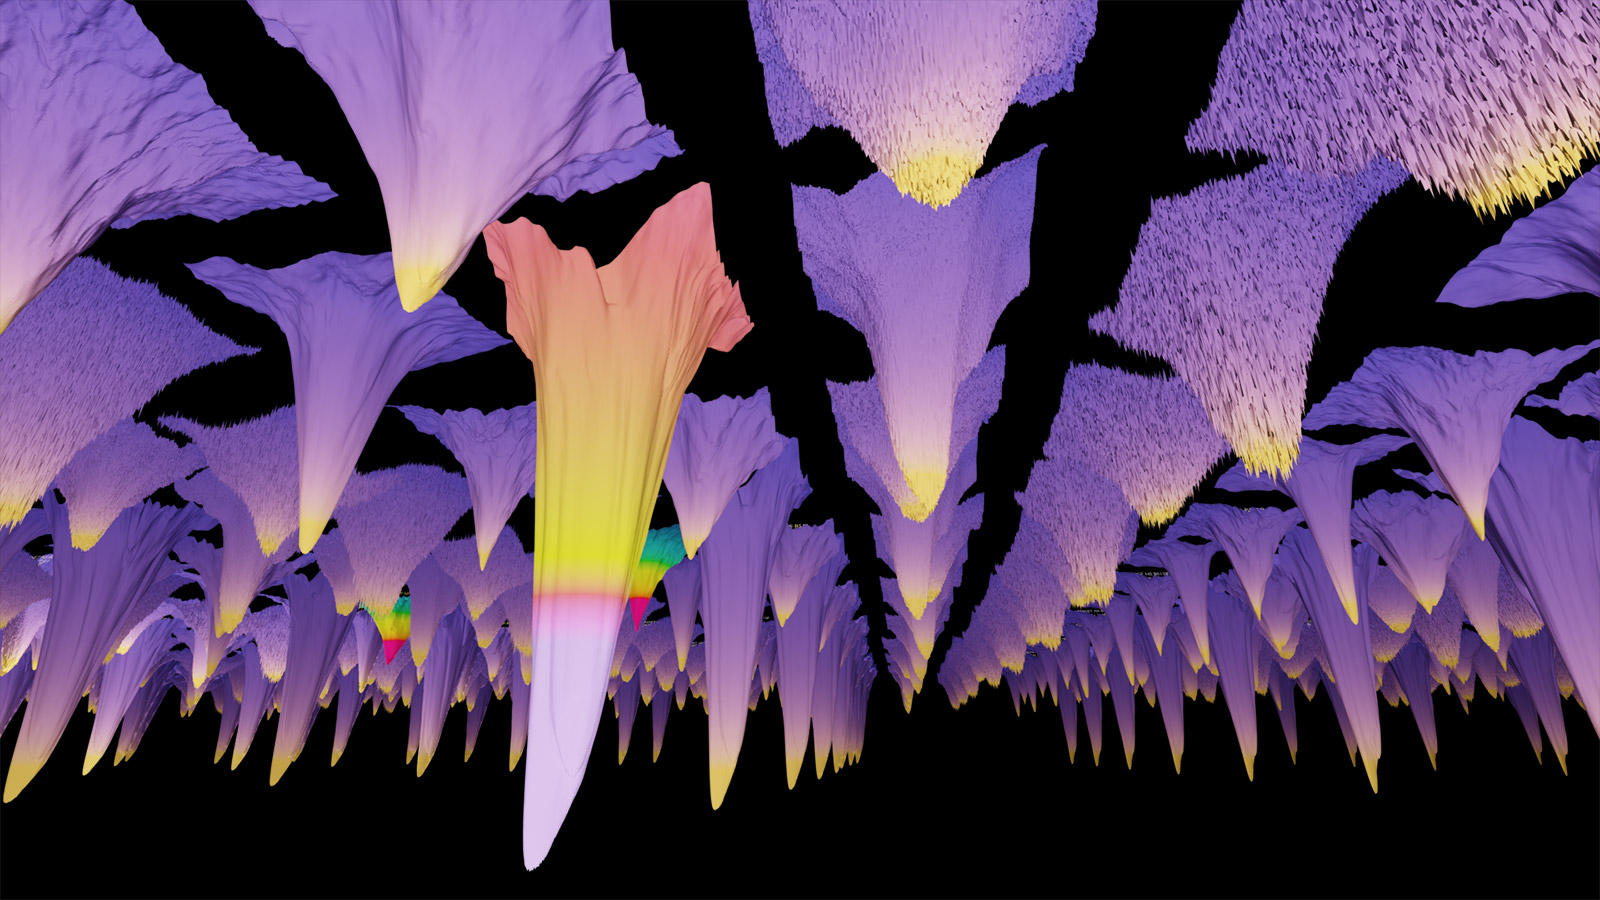
\includegraphics[trim={0cm 0cm 0cm 0cm},clip]{loss2.jpg}}
       \end{center}
    \end{figure}

    Source: \url{https://losslandscape.com/gallery/}

\end{frame}




\begin{frame}
    \frametitle{How does it work?}
    
    Why is it possible to minimize over $\theta \in \RR^d$ when $d=10^{12}$ ?!?

        \vspace{0.5em}
        \vspace{0.5em}
        \vspace{0.5em}
        \vspace{0.5em}
        \pause

    Core elements
    %
    \begin{itemize}
        \item automatic differentiation (for \underline{gradient} descent)
        \vspace{0.5em}
        \item parallelization (GPUs or TPUs)
        \vspace{0.5em}
        \item Compilers / JIT-compilers
    \end{itemize}

\end{frame}

\begin{frame}[fragile]
    \frametitle{Automatic differentiation}

    \vspace{0.5em}
    ``Exact numerical'' differentiation
    
    \begin{minted}{python}

def loss(θ, x, y):
  return jnp.sum((y - f(θ, x))**2)

loss_gradient = grad(loss)

    \end{minted}

    \vspace{0.5em}
    \vspace{0.5em}
    \vspace{0.5em}
    Now use gradient descent\ldots


\end{frame}


\begin{frame}[fragile]
    \frametitle{Parallelization}

    \begin{figure}
       \begin{center}
        \scalebox{0.18}{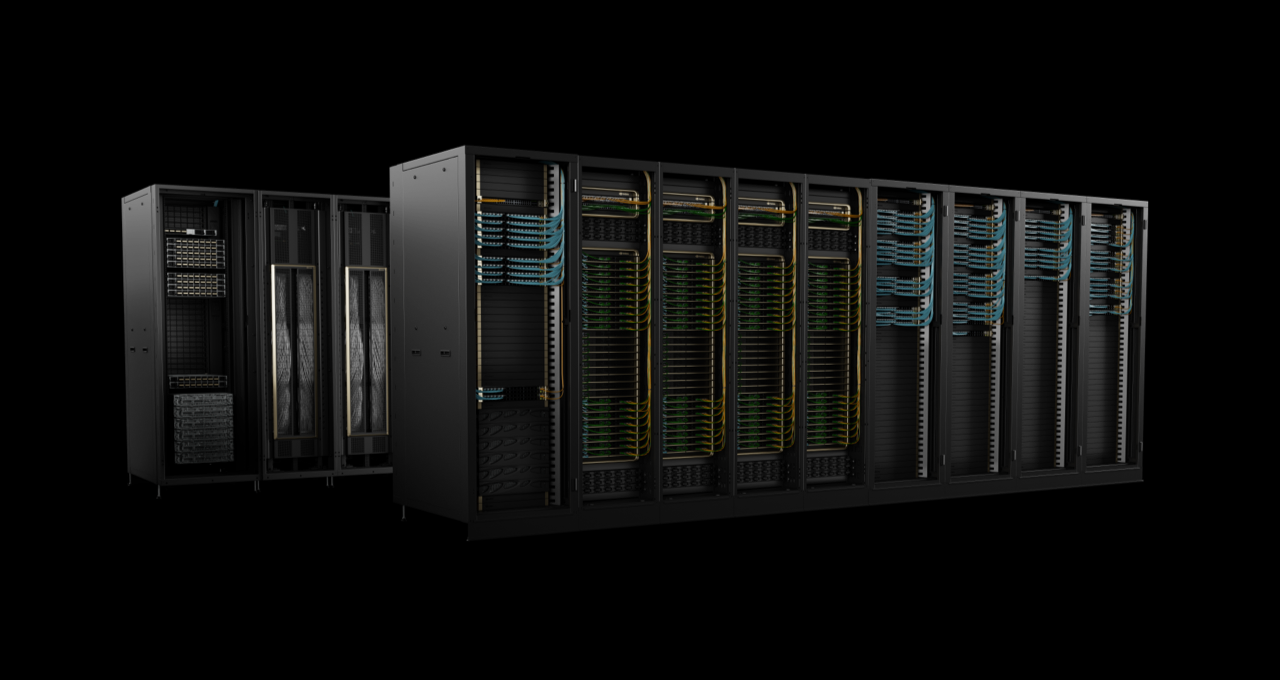
\includegraphics[trim={0cm 0cm 0cm 0cm},clip]{dgx.png}}
       \end{center}
    \end{figure}
    
\end{frame}


\begin{frame}[fragile]
    
    \begin{minted}{python}
outputs = pmap(f, data)  
    \end{minted}

    \vspace{0.5em}
    \vspace{0.5em}
    \begin{itemize}
        \item multithreading over GPU cores (how many?)
        \vspace{0.5em}
        \item multiprocessing over accelerators in a GPU farm / supercomputing
            cluster (how many?)
    \end{itemize}

\end{frame}


\begin{frame}[fragile]
    \frametitle{Just-in-time compilers}

    \vspace{0.5em}
    
    \begin{minted}{python}
@jit
def f(x):
    return jnp.sin(x) - jnp.cos(x**2)
    \end{minted}

    \vspace{0.5em}
    Advantages over AOT compilers:

    \begin{itemize}
        \item cleaner code
    \vspace{0.5em}
        \item more portable
    \vspace{0.5em}
        \item automatic parallelization (same code for CPUs / GPUs)
    \end{itemize}

\end{frame}


\begin{frame}
    
    Advantages over NumPy / MATLAB

    \vspace{0.5em}
    \begin{itemize}
        \item can specialize machine code based on parameter types / shapes
        \vspace{0.5em}
        \item automatically matches tasks with accelerators (GPU / TPU)
        \vspace{0.5em}
        \item fuses array operations for speed and memory efficiency
    \end{itemize}

\end{frame}


\begin{frame}
    \frametitle{Platforms}
    
    Platforms that support AI / deep learning:

    \vspace{0.5em}
    \begin{itemize}
        \item Tensorflow
        \vspace{0.5em}
        \item \brown{PyTorch} (Llama, ChatGPT)
        \vspace{0.5em}
        \item \brown{Google JAX} (Gemini, DeepMind)
        \vspace{0.5em}
        \item Keras (backends $=$ JAX, PyTorch)
        \vspace{0.5em}
        \item Mojo? (Modular (Python))
        \vspace{0.5em}
        \item MATLAB? 
    \end{itemize}

\end{frame}




\begin{frame}
    
    Popularity -- languages
    
    \begin{figure}
       \begin{center}
        \scalebox{0.62}{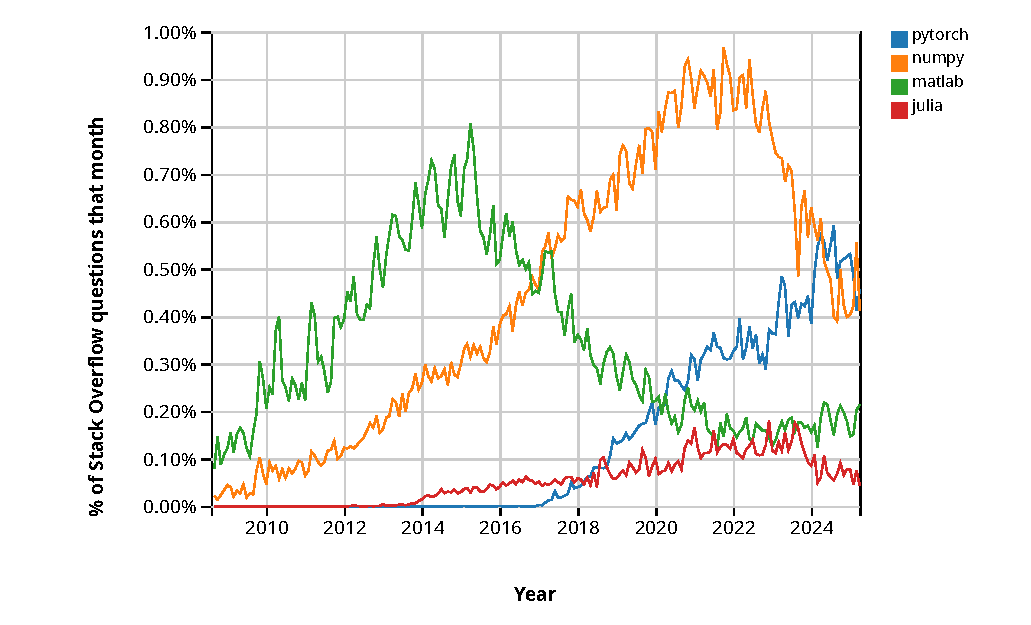
\includegraphics[trim={0cm 0cm 0cm 0cm},clip]{trends.pdf}}
       \end{center}
    \end{figure}

\end{frame}


\begin{frame}
    
    Popularity -- deep learning frameworks
    
    \begin{figure}
       \begin{center}
        \scalebox{0.62}{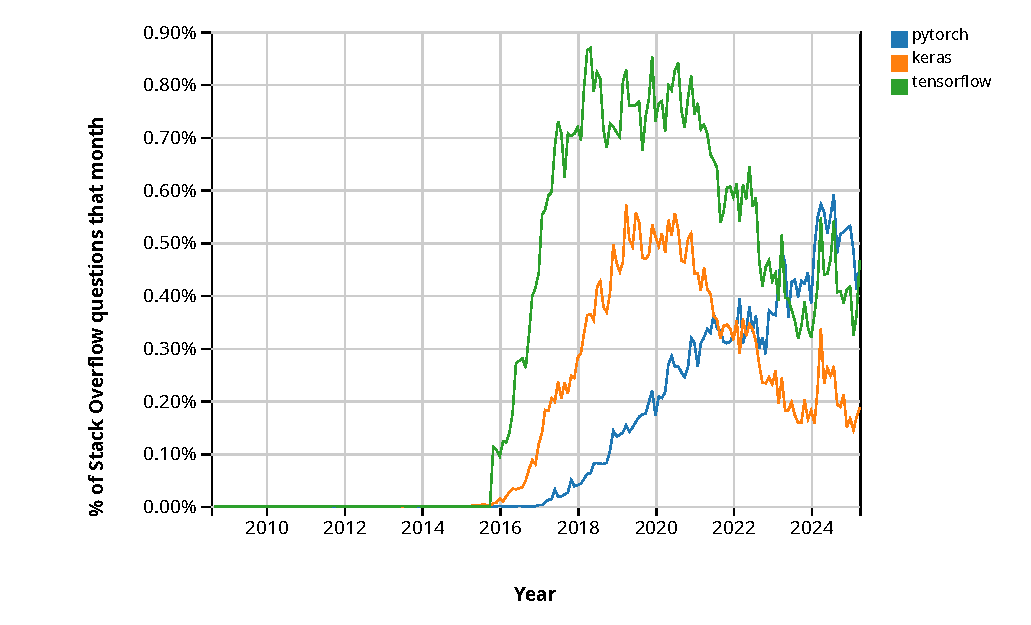
\includegraphics[trim={0cm 0cm 0cm 0cm},clip]{trends_2.pdf}}
       \end{center}
    \end{figure}

\end{frame}


\begin{frame}
    \frametitle{AI tools for economic modeling}

    Let's say that you want to do computational economics without deep learning

    \vspace{0.5em}
    Can these new AI tools be applied?

    \pause

    \vspace{0.5em}
    \vspace{0.5em}
    \emp{Yes!}
    \emp{Yes!}
    \emp{Yes!}

    \begin{itemize}
        \item fast matrix algebra
        \vspace{0.5em}
        \item fast solutions to linear systems
        \vspace{0.5em}
        \item fast nonlinear system solvers
        \vspace{0.5em}
        \item fast optimization, etc.
    \end{itemize}


\end{frame}



\begin{frame}
    \frametitle{Case Study}

    The CBC uses the ``overborrowing'' model of Bianchi (2011)

    \begin{itemize}
        \item credit constraint loosens during booms
        \item bad shocks $\to$ sudden stops
    \end{itemize}

    \vspace{0.5em}
    CBC implementation in MATLAB 

    \begin{itemize}
        \item runs on \$10,000 mainframe with 356 CPUs and 1TB RAM
        \item runtime $=$ 12 hours
    \end{itemize}

    \pause
    \vspace{0.5em}
    Rewrite in Python + Google JAX

    \begin{itemize}
        \item runs on \$400 gaming GPU with 10GB RAM
        \item runtime $=$ 7 seconds
    \end{itemize}


\end{frame}




\end{document}


